
\documentclass[12pt]{article}
\usepackage{graphicx} % for including images
\usepackage{hyperref} % for creating hyperlinks
\usepackage{amsmath} % for mathematical expressions
\usepackage{lipsum} % for generating dummy text
\usepackage{listings} % for code blocks
\usepackage{float} % place images where they appear in the LaTeX
\usepackage{pdfpages} % insert PDFs in the document

\lstset{
  language=bash,
  basicstyle=\ttfamily,
  breaklines=true
}

\begin{document}
% Title page information
\title{Sound Classification and Localization by Acoustic Sensing on Raspberry Pi 4}
\author{Jaidon Lybbert, University of Washington}
\date{January 24, 2024}

% Generate the title page
\maketitle

% Abstract section
\begin{abstract}
	In this article a network of distributed acoustic sensing nodes is used to localize a sound signature using a time-difference-of-arrival (TDoA) algorithm. Accurate wall-clock times are obtained by GPS at each node, and a frame of acoustic data is recorded through a microphone on each node. Time differences are determined by correlation, and the resulting system of equations solved by the Chan-Ho algorithm to determine location. In a concurrent process, each node performs classification inference on a data frame using a pre-trained convolutional neural network (CNN). The resulting class identification is used to assign a process model to the tracked object for use in an Extended Kalman Filter (EKF) applied to the Chan-Ho localization result to make the final estimate of object position and trajectory.
\end{abstract}

% Introduction section
\section{Introduction}
This document is organized as follows. In Section \ref{sec:background} \ref{sec:methods} \ref{sec:results} \ref{sec:discussion}. I conclude in \ref{sec:conclusion} by discussing the overall takeaways from my experiments and things I would like to try in the future.

% Methods section
\section{Background}\label{sec:background}



\section{Kalman Filters}

	The Extended Kalman Filter (EKF) is a well-described algorithm, where discrete samples from one or more sensors is combined with an analytic model of a system to estimate system state. A block diagram of the Kalman Filter from \textit{Kalman Filters for Beginners} by Phil Kim \cite{kim2011kalman} is shown in Fig \ref{fig:kimkalman}.
	
\begin{figure}[h]
\centering
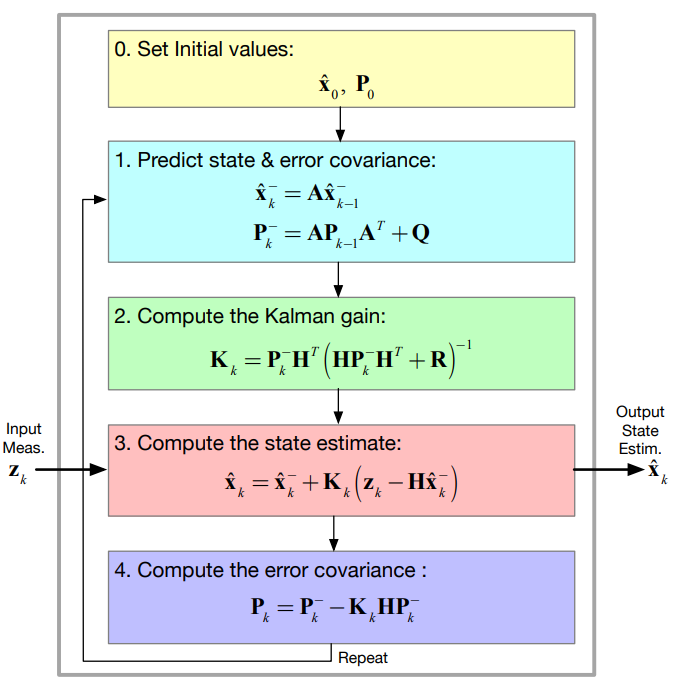
\includegraphics[width=0.5\textwidth]{kimkalman.png} % replace with your own image file
\caption{Block diagram of the Kalman Filter algorithm. $\hat{\mathbf{x}}_0$ represents the initial state.}
\label{fig:kimkalman}
\end{figure}

\section{Methods}\label{sec:methods}

\subsection{Environment Setup}

	For classification, I will be using TensorFlow Lite
	
\subsection{TensorFlow Lite}
	TensorFlow Lite (TFLite) is a lightweight version of the TensorFlow runtime for loading machine learning models and running inference on input data. TFLite runs on resource-constrained devices like the Raspberry Pi. I use TFLite for loading a pretrained model for classification of bird species by sound. The model of choice is taken from the BirdNET project, and contains 6,000 species. The input to the model is a 3 second long frame of audio sampled at 48kS/s, and the output is an 6k element array containing the class estimates. The model has a secondary input which takes in latitude, longitude, and the week of the year (1-52).
	
	I first referenced the TFLite Python API documentation to attempt loading the model, and running it against a sample audio clip. I quickly found out that the high-level API and provided binaries for the \textbf{aarch64} architecture are not well supported by the TensorFlow developers. I shifted my strategy to setting up the BirdNET-Pi project to run on my device. I ran into build and dependency issues, since the developers of the BirdNET-Pi project support a previous release of the Raspberry Pi OS. Instead of re-installing a different OS, I used the source code of BirdNET-Pi as reference to write a minimally working script to get TFLite working on the Pi.
	
	The BirdNET model contains functions that require a piece of software to be compiled in with the TFLite binary. This runtime is not available in the binary provided by the TFLite developers, so I used a version provided by an independent developer who compiles the runtime with this software for the Pi. The TFLite wheel was incompatible with the system installation of Python 3.11 included in the Raspberry Pi OS. I installed \textbf{pyenv} to install Python 3.9 and manage the two different versions. The versions of packages required by the TFLite wheel, such as \textbf{Numpy} were incompatible with the versions installed by \textbf{pip} by default, and changing the version manually broke dependency rules for other packages like \textbf{matplotlib}. I created a \textbf{requirements.txt} file for \text{pip}, and manually wrote the dependency rules  to get all packages working.
	
	I took a sample audio \textbf{MP3} of a known bird species from an online database, and loaded it into Python with \textbf{pydub}, and converted it to a \textbf{Numpy} array. I wrote a function to split the file into 3 second chunks. For each chunk, I put the array of samples into the first TFLite input tensor, and put the location and time data into the second input tensor. I timed how long it took for inference, and recorded the estimate result. I plotted the inference execution time over all frames of audio.
	
\subsubsection{GPS}
	I used the Adafruit Ultimate GPS USB breakout board to get GPS data through \textbf{gpsd} \cite{townsend2023}. \textbf{gpsd} is a Linux daemon which listens on port 2497 of the loopback address by default. When a connection request is recieved, it begins communicating with the GPS module over USB by reading data through the /dev/ttyUSB0 device file, and forwarding it to the TCP/IP port to service the request. By default, \textbf{gpsd} is managed through \textbf{systemd}. Adafruit recommends disabling this functionality through the \textbf{systemctl} interface, and running \textbf{gpsd} manually.
	
\begin{lstlisting}
sudo apt install gspd gpsd-clients
sudo systemctl stop gpsd.socket
sudo systemctl disable gpsd.socket
sudo killall gpsd
sudo gpsd /dev/ttyUSB0 -F /var/run/gpsd.sock
\end{lstlisting}

To test the device I used the command \textbf{cgps -s}, which is a \textbf{gspd} client that communicates over the default port and prints out GPS status information to the console, as shown in Fig. \ref{fig:cgps}. It took significant troubleshooting to get this to work properly. What I finally determined to work was editing the configuration of \textbf{gpsd} defined in the \textbf{/etc/default/gpsd} file, and rebooting. 

\begin{lstlisting}
DEVICES=""
START_DAEMON="true"
GPSD_OPTIONS="/dev/ttyUSB0 -G"
USBAUTO="true"
GPSD_SOCKET="/var/run/gpsd.sock"
\end{lstlisting}

The other necessary step was physically moving my test setup from the basement to the main floor of my house, since I could not get a reliable connection to the GPS satellites from the basement.

Once I had a reliable connection, I wrote a Python script to collect about 1200 GPS readings of latitude and longitude, while leaving the system stationary, and wrote the readings to a \textbf{.csv} file. I wrote a script to convert degrees of latitude and longitude to meters, then plotted a histogram of the differences of each reading from the mean value to evaluate the spatial precision of the GPS reciever.

\begin{figure}[h]
\centering
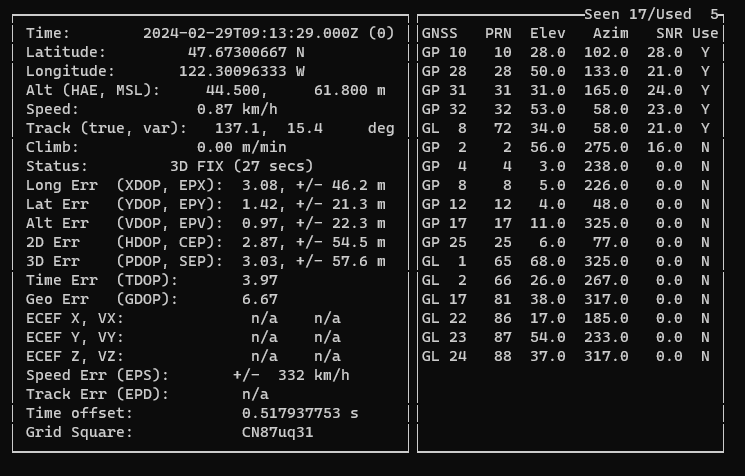
\includegraphics[width=0.8\textwidth]{cgps.png} % replace with your own image file
\caption{Terminal display of GPS information from the \textbf{cgps -s} command.}
\label{fig:cgps}
\end{figure}

\subsection{Microphone}
	I use an generic adjustable-gain microphone module to sample the acoustic signals with the ESP8266 sensing node. For my breadboard prototype, I don't have an ADC capable of sampling at the 48kS/s rate required by the TFLite model. Given more time, I would implement the Analog Devices SSM2603 audio CODEC, which has programmable gain and a digital I2S interface. 
	I power the microphone with 3.3V from an ELEGOO breadboard power supply connected to a wall outlet through a 9V wall wart. The microphone output is connected to a simple first-order low-pass antialiasing filter implemented with a resistor and capacitor on the breadboard with a cutoff frequency of 20kHz. The output of the filter is connected to an ADC on the ESP8266.
	To characterize the microphone noise, I tape over the transducer, then sample the ADC with the ESP8266, and send the samples over to the Raspberry Pi through the web socket interface. I record the samples to a \textbf{CSV} to plot the sample distribution.

\subsection{ESP8266}
	Each acoustic sensing node is implemented as an Adafruit Feather HUZZAH ESP8266 MCU which connects to a common WiFi network and communicates with the Raspberry Pi through web sockets. For my prototype, the ESP8266 is connected to my home router. 
	The EEPROM of the ESP8266 is flashed with the MicroPython runtime through a micro-USB cable connected to my laptop using the \textbf{esptool} CLI. Configuration of the ESP8266 can be done through the read-evaluate-print-loop (REPL) accessed through a serial port using PuTTY. MicroPython automatically executes the \textbf{boot.py} script in the ESP filesystem when the device is powered on, then executes \textbf{main.py}.
	In order to edit the scripts on the ESP8266, I use the \textbf{Ampy} command line tool created by Adafruit to modify the filesystem over the serial port. Ampy can be installed through \textbf{pip}, then commands can be issued to copy files over by specifying the serial port.
	I wrote a script \textbf{server.py} which is loaded onto the ESP. The script opens a web socket and listens for a connection from the Raspberry Pi, which . When the connection is made, the ESP begins sampling the ADC and stores the samples into a buffer. The buffer is sent over the connection to be recieved by the Raspberry Pi.


\subsection{Simulator}
	The effectiveness of localization based on acoustic signals depends on factors including:
	
\begin{itemize}
  \item Sensor noise
  \item Environment noise
  \item Sampling quantization
  \item Sensor and source geometry
  \item Sound speed
  \item Reverberation
\end{itemize}

	In order to test my localization algorithm under variation of these parameters, I created a simple simulator in Python to place sensors and sources spatially in the environment, add noise to the signal, simulate the sound propogating from source to each listening sensor, and visualize the resulting hyperbolas of the TDE algorithm and the localization result. The simulator uses the \textbf{Pygame} library to graphically represent the environment.
	

\subsection{Time-Difference Estimation (TDE)}
	To develop the TDE algorithm, I use the simulated time-shifted inputs, and apply simple correlation using the \textbf{scipy} Python library. The peak of the digital correlation result between signals recieved at two nodes is used to determine the number of samples the signal is delayed by at one node compared to the other. Based on the sample rate, the time delay is determined.
	I iterate through all audio frames and compute TDE for each simulated node-pair. The resulting TDEs will be used in the localization algorithm to determine the localization result. I profile the execution time of the TDE algorithm, and write the output to a \textbf{csv} file for plotting.
	
\subsection{Localization Estimate}
	The set of TDEs define a system of hyperbolic equations. When there are exactly 3 TDEs, the equations are represented by a singular matrix, with one solution. With more than 3 TDEs, the matrix is overdetermined, and a least-squares method is necessary to make the final localization estimate. Least-squares is a complicated algorithm to optimize, but well studied, with implementations using matrix decomposition techniques. For this project, I use the \textbf{Numpy} Python library, which under the hood, calls a compiled system BLAS library written in C located at \textbf{/usr/lib/aarch64-linux-gnu/blas}, and the compiled LAPACK library written in FORTRAN 77 located at {/usr/lib/aarch64-linux-gnu/lapack}. My profiling tests in the characterization process showed that these implementations take advantage of the Advanced SIMD architecture of the Cortex-A72 CPU for doing tensor operations, and vastly outperformed my best attempts at matrix multiplication in Rust.

\subsection{Fast Fourier Transform}
	The correlation algorithm I used is very basic, but falls short in the real-world where correlated noise like wind and reverberation exists in the signals. The majority of studied localization algorithms use a variation of the Generalized Cross-Correlation Phase Transform (GCC-PHAT) algorithm. Which transform the signal to the frequency domain using the Fast Fourier Transform. For this project, I didn't have time to implement a more complicated localization algorithm, but I did profile the FFT algorithm provided by the Numpy and SciPy libraries to evaluate the CPU time it would require, since the FFT accounts for the majority of required FLOPs in these algorithms. 

% Results section
\section{Results}\label{sec:results}

% Discussion section
\section{Discussion}\label{sec:discussion}

% Conclusion section
\section{Conclusion}\label{sec:conclusion}

\paragraph{Note}
\textit{All my code and project files for this and future reports, can be found on my GitHub repository \cite{lybbert2024classwork}.}

% Bibliography from refs.bib
\bibliographystyle{plain}
\bibliography{refs}

\end{document}
